%%%%%%%%%%%%%%%%%%%%%%%%%%%%%%%%%%%%%%%%%%%%%%%%%%%%%%
% A Beamer template for Ritsumeikan University       %
% Author: Ming-Hao Xu (Xu Minghao)                   %
% Date:   April 2022.                                %
% LPPL Licensed.                                     %
%%%%%%%%%%%%%%%%%%%%%%%%%%%%%%%%%%%%%%%%%%%%%%%%%%%%%%

\documentclass{beamer}
\usepackage{hyperref}

\usepackage[UTF8]{ctex}
\usepackage[T1]{fontenc}

% other packages
\usepackage{latexsym,amsmath,xcolor,multicol,booktabs,calligra}
\usepackage{graphicx,pstricks,listings,stackengine}
\usefonttheme[onlymath]{serif}

% dummy text; remove it when working on this template
\usepackage{lipsum}

\author{Ebola}
\title{字符串进阶:AC自动机}
\institute{
    Institute of Mathematics, \\
    Zhejiang University.
}
\date{Jan, 2024}
\usepackage{Ritsumeikan}

% defs
\def\cmd#1{\texttt{\color{red}\footnotesize $\backslash$#1}}
\def\env#1{\texttt{\color{blue}\footnotesize #1}}
\definecolor{deepblue}{rgb}{0,0,0.5}
\definecolor{deepred}{rgb}{0.6,0,0}
\definecolor{deepgreen}{rgb}{0,0.5,0}
\definecolor{halfgray}{gray}{0.55}

\lstset{
    basicstyle=\ttfamily\tiny,
    keywordstyle=\bfseries\color{deepblue},
    emphstyle=\ttfamily\color{deepred},    % Custom highlighting style
    stringstyle=\color{deepgreen},
    numbers=left,
    numberstyle=\small\color{halfgray},
    rulesepcolor=\color{red!20!green!20!blue!20},
    frame=shadowbox,
}


\begin{document}

\begin{frame}
    \titlepage
\end{frame}

\begin{frame}
    \tableofcontents[sectionstyle=show,subsectionstyle=show/shaded/hide,subsubsectionstyle=show/shaded/hide]
\end{frame}

\section{基础回顾}

\begin{frame}{字典树(Trie)}
    \small

    字典树把所有的字符串存储在一棵树中,
    可以方便地查询所有的前缀。

    \vspace{1em}
    我们来回顾一下字典树模板题。
\end{frame}

\begin{frame}[fragile]{字典树(Trie)}
    \small

    插入操作
    \begin{lstlisting}[language=c++]
int mapping(char c){
    if(c>='A' && c<='Z') return c-'A';
    else return c-'a'+26;
}
void insert(char s[]){
    int n = strlen(s+1);
    int cur = 0;
    sz[0]++;
    for(int i = 1; i <= n; i++){
        int j = mapping(s[i]);
        if(ch[cur][j]==0){
            ch[cur][j] = tot;
            tot++;
        }
        cur = ch[cur][j];
        sz[cur]++;
    }
}
    \end{lstlisting}
\end{frame}

\begin{frame}[fragile]{字典树(Trie)}
    \small

    查询操作
    \begin{lstlisting}[language=c++]
int query(char s[]){
    int cur = 0;
    int n = strlen(s+1);
    for(int i = 1; i <= n; i++){
        int j = mapping(s[i]);
        if(ch[cur][j]==0) return 0;
        cur = ch[cur][j];
    }
    return sz[cur];
}
    \end{lstlisting}
\end{frame}

\begin{frame}{最大异或和问题}
    \small

    最大异或和问题是 Trie 的一个经典应用。

    \vspace{1em}
    给定 $n\;(\leq 10^5)$ 个数,所有数均不超过 $2^{31}-1$.
    从中选两个数,使它们异或起来最大。 
\end{frame}

\begin{frame}{最大异或和问题}
    \small

    把所有的数都转化为 $31$ 位二进制数,高位不足则补零,
    然后把二进制数当成字符串插入进 Trie 中。

    \vspace{1em}\pause
    现在,我们枚举 $x=a_i\;(i=1,...,n)$,来找一个数 $a_j$,使它和 $x$ 异或起来最大。

    \vspace{1em}\pause
    从高位到低位贪心,尽可能让异或和的高位为 $1$。例如:
    如果 $x$ 最高位是 $0$,那么我们希望选出的 $a_j$ 最高位是 $1$,
    这样异或起来最高位才会是 $1$,因此我们第一步从 Trie 的根节点
    往 $1$ 的方向走。
\end{frame}

\begin{frame}[fragile]{最大异或和问题}
    \small

    总之,如果 $x$ 的第 $k$ 位是 $x_{k}$,那么这一步就尽量往 $x_{k}\;\text{xor}\; 1$
    方向走,除非 Trie 不存在对应的分支,此时不得不往 $x_{k}$ 走。
    最后代码像这样:
    \begin{lstlisting}[language=c++]
int query(int x){
    int cur = 0;
    const int n = 31;
    for(int i = 1; i <= n; i++){
        int j = (x >> (31-i)) & 1;
        if(ch[cur][j^1]==0) cur = ch[cur][j];
        else cur = ch[cur][j^1];
    }
    return val[cur];
}
    \end{lstlisting}
\end{frame}

\begin{frame}[fragile]{第 k 大异或和问题}
    \small

    如果想对于给定的 $x$,找到一个 $a_i$,使 $x\oplus a_i$ 是
    $x\oplus a_1,...,x\oplus a_n$ 中第 $k$ 大的数,应该如何写?

    \pause
    \begin{lstlisting}[language=c++]
int query(int x, int k)
{
    int o=1;
    int res=0;
    for(int i=31;i>=0;i--)
    {
        int j=(x>>i)&1;
        if(sz[ch[o][j^1]]>=k) o=ch[o][j^1],res|=1u<<i;
        else k-=sz[ch[o][j^1]],o=ch[o][j];
    }
    return res;
}
    \end{lstlisting}
\end{frame}

\begin{frame}[fragile]{[十二省联考 2019] 异或粽子}
    \small

    给定 $n\;(\leq 5\times 10^5)$ 个数 $a_1,...,a_n$,选一个区间 $[l,r]$,将 $a_l,...,a_r$ 全部异或起来,
    得到这个区间的权值。求权值前 $m\;(\leq 2\times 10^5)$ 大的区间权值之和。
\end{frame}

\begin{frame}[fragile]{[十二省联考 2019] 异或粽子}
    \small

    令 $b_i=a_1\oplus...\oplus a_i$,那么 $a_l\oplus...\oplus a_r=b_{l-1}\oplus b_r$,转化为两个数的异或,
    可以用 Trie 解决。

    \vspace{1em}\pause
    具体地,先把 $b_0,...,b_n$ 的二进制插入 Trie 中。
    接下来对每个 $b_i$ 找到一个 $b_j$ 使它和 $b_i$ 异或起来最大。

    \vspace{1em}\pause
    将这些值存进一个优先队列中。每次从优先队列取出最大的异或和,弹出,
    如果它是 $b_i$ 和其它数的异或和中第 $k$ 大的,
    就找到 $b_i$ 和其它数的异或和中第 $k+1$ 大的加入优先队列。
    不断重复,直到弹出的数达到 $2m$ 个为止,最后答案要除以 $2$. (为什么?)
\end{frame}

\section{AC自动机}

\begin{frame}[fragile]{基本概念}
    \small
    AC自动机 = 字典树 + fail数组

    \vspace{1em}
    对所有模式串建立字典树,根节点为 $0$ 号。
    
    \vspace{1em}\pause
    设 $p$ 是字典树上的一个节点,从根节点到 $p$ 的路径上所有的字母拼起来一定是某个模式串的前缀,我们记这个前缀为 $S_p$,我们说它是 $p$ 代表的字符串
    
    \vspace{1em}\pause
    \verb|fail[p]| 是字典树的一个节点,而且它代表的前缀也是 $S_p$ 的后缀,并且是最长的那个。\pause 用数学语言就是:
    
    \begin{equation*}
        \mathcal{F}(p)=\{q \;|\; q \text{是节点,满足} q\neq p \text{,且} S_q \text{是} S_p \text{的后缀}\}
    \end{equation*}
    
    \begin{equation*}
        fail[p]\in\mathcal{F}(p),\quad \text{且} \;|S_{fail[p]}| = \max_{q\in \mathcal{F}(p)} |S_q|
    \end{equation*}
    
    \pause 特别地,如果 $\mathcal{F}(p)=\varnothing$,那么 $fail[p]=0$。
\end{frame}

\begin{frame}[fragile]{fail 树}
    \small
    如果把每个节点 $p$ 向 $fail[p]$ 连一条蓝色的边,
    我们会发现,所有蓝色的边构成一棵树,其中 $p$ 的父亲是 $fail[p]$.

    \begin{figure}[H]
        \centering
        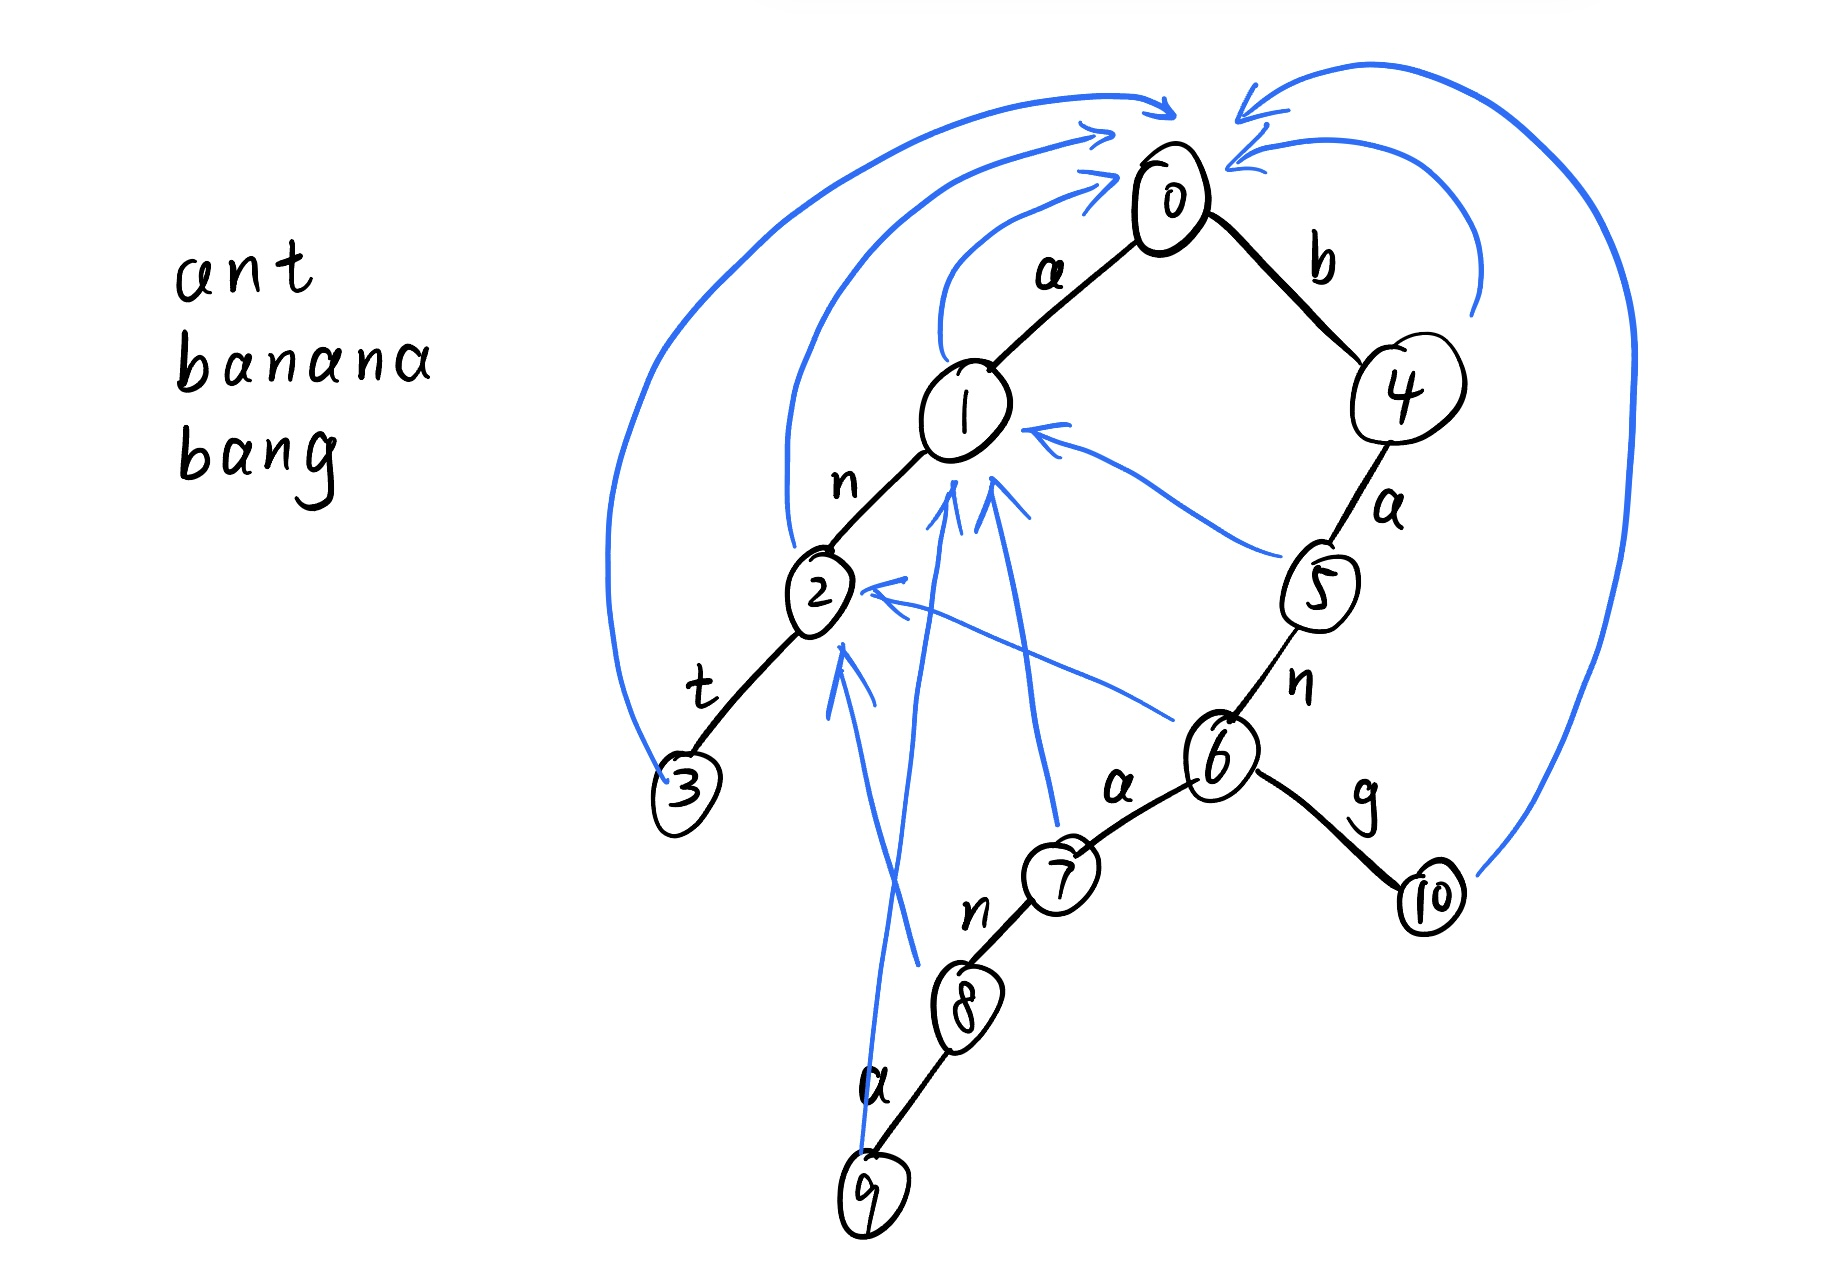
\includegraphics[width=0.8\textwidth]{pic/fail.jpg}
    \end{figure}

    \vspace{1em}\pause
    如果我们想找到所有 $\mathcal{F}(p)$ 中的节点,
    只需要沿着 fail 树一直往上跳即可。
\end{frame}

\begin{frame}[fragile]{求 fail}
    \small
    现在,我们来看如何求 \verb|fail| 数组。
    注意,必须先把所有模式串的字典树建立好,才能开始求 \verb|fail|。

    \vspace{1em}\pause
    我们用字典树的 BFS 序来求 \verb|fail|,现在遍历到节点 \verb|u|,我们
    来枚举它的下一个节点 \verb|v=ch[u][c]|。
    
    \vspace{1em}\pause
    试想,如果 \verb|fail[v]| 不指向根,那么 \verb|fail[v]=q|,其中 \verb|q=ch[f][c]|(一定存在这样的 $f$)。
    这个 \verb|f| 在哪里找?

    \vspace{1em}\pause
    显然,$f\in \mathcal{F}(u)$,因此只要从 $u$ 出发,沿着 fail 树往上跳,如果
    发现某个 \verb|f| 满足 \verb|ch[f][c]|$\neq 0$ 就立刻停止,并令 \verb|fail[v]=ch[f][c]|。
\end{frame}

\begin{frame}[fragile]{求 fail}
    \small
    \begin{lstlisting}[language=c++]
void getfail(){
    queue<int> q;
    for(int c = 0; c < 26; c++)
        if(ch[0][c]) q.push(ch[0][c]);
    while(!q.empty()){
        int u = q.front(); q.pop();
        for(int c = 0; c < 26; c++){
            int v = ch[u][c];
            if(!v) continue;
            int f = fail[u];
            while(f && !ch[f][c]) f = fail[f];
            fail[v] = ch[f][c];
            q.push(v);
        }
    }
}
    \end{lstlisting}

    它是 $O(n)$ 的,为什么?
\end{frame}

\begin{frame}[fragile]{[P3808] AC自动机(简单版)}
    \small
    给定 $n$ 个模式串 $s_i$ 和一个文本串 $t$,求有多少个不同的模式串在文本串里出现过。  

    两个模式串不同当且仅当他们 \textbf{编号} 不同。
\end{frame}

\begin{frame}[fragile]{[P3808] AC自动机(简单版)}
    \footnotesize

    首先构建模式串的字典树,并求出 fail 数组。

    \vspace{.7em}\pause
    现在,我们在字典树上从根节点出发,顺着文本串 $s$ 一步一步走,即
    \verb|u=0|,\verb|u=ch[u][s[1]]|,\verb|u=ch[u][s[2]]|,……
    (我们先假设不会碰到走不下去的情况)

    \vspace{.7em}\pause
    可以知道,在这个过程中,$S_u$ 都在 $s$ 中出现过;$S_p\;(p\in \mathcal{F}(u))$
    也都在 $s$ 中出现过;除此之外不会有其它的出现过。

    \vspace{.7em}\pause
    这就产生了一种做法:令 \verb|appear[u]| 表示 $S_u$ 是否在 $s$ 中出现过,
    $u$ 每走一步,就把 \verb|appear[u]| 标记成 \verb|true|;然后令 $f$ 从 $u$
    出发,沿着 fail 一直跳到根,把途径的 \verb|appear[f]| 都标记成 \verb|true|.

    \vspace{.7em}\pause
    当然,在 $f$ 往上跳的过程中,如果发现 \verb|appear[f]| 已经被标记成了 \verb|true|,
    那么可以立即终止循环,因为之后的肯定早就被标记过了。这样可以保证
    fail 树上的每个节点只被标记一次,从而保证复杂度线性。

    \vspace{.7em}\pause
    现在,如果 $u$ 在走的过程中发现走不下去,怎么办?

    \vspace{.7em}\pause
    沿着 fail 往上跳,直到 \verb|ch[u][s[i]]|$\neq 0$ 为止。
    (请思考:为什么这样能保证不重不漏地标记在 $s$ 中出现过的所有 $S_p$)
\end{frame}

\begin{frame}[fragile]{[P3808] AC自动机(简单版)}
    \small
    代码像这样:

    \begin{lstlisting}[language=c++]
void traval(char s[]){
    int n = strlen(s+1), u = 0;
    for(int i = 1; i <= n; i++){
        int c = s[i] - 'a';
        while(u && !ch[u][c]) u = fail[u];
        u = ch[u][c];
        appear[u] = true;
        int f = fail[u];
        while(f && !appear[f])
            appear[f] = true, f = fail[f];
    }
}
    \end{lstlisting}

    \vspace{1em}\pause
    在字典树 insert 的过程中,记录一下每一个模式串 $t_i$ 对应的节点是哪个,
    记作 \verb|idx[i]|,然后根据 \verb|appear[idx[i]]| 来统计答案。
\end{frame}

\begin{frame}[fragile]{求 fail(路径压缩版)}
    \small
    我们可以在求 fail 的时候顺便压缩路径。

    \vspace{1em}\pause
    具体而言,因为我们知道在 traval 的过程中,
    如果发现 \verb|ch[u][c]=0|,我们会从 $u$ 出发沿着 fail 往上跳,
    直到找到 \verb|ch[f][c]=q|$\neq 0$ 的位置为止。
    我们不妨在求 fail 的时候就把这一步做好,一步到位令 \verb|ch[u][c]=q|.

    \pause
    \begin{lstlisting}[language=c++]
void getfail(){
    queue<int> q;
    for(int c = 0; c < 26; c++)
        if(ch[0][c]) q.push(ch[0][c]);
    while(!q.empty()){
        int u = q.front(); q.pop();
        int f = fail[u];
        for(int c = 0; c < 26; c++){
            int& v = ch[u][c];
            if(!v) v = ch[f][c];
            else fail[v] = ch[f][c], q.push(v);
        }
    }
}
    \end{lstlisting}
\end{frame}

\begin{frame}[fragile]{搜索(路径压缩版)}
    \small
    有了路径压缩,我们在 travel 的过程中就不需要跳 fail 了。
    (当然,标记答案的时候还是要跳 fail)

    \begin{lstlisting}[language=c++]
void traval(char s[]){
    int n = strlen(s+1), u = 0;
    for(int i = 1; i <= n; i++){
        int c = s[i] - 'a';
        u = ch[u][c];
        appear[u] = true;
        int f = fail[u];
        while(f && !appear[f])
            appear[f] = true, f = fail[f];
    }
}
    \end{lstlisting}
\end{frame}

\begin{frame}[fragile]{[P5357] 【模板】AC自动机}
    \small
    给定 $n$ 个模式串 $s_i$ 和一个文本串 $t$,求每个模式串在文本串里出现的次数。  
\end{frame}

\begin{frame}[fragile]{[P5357] 【模板】AC自动机}
    \footnotesize
    我们回顾之前的 travel 代码,很容易会想把 \verb|appear| 数组改成
    \verb|cnt| 数组,用于统计出现次数,像这样:

    \begin{lstlisting}[language=c++]
void traval(char s[]){
    int n = strlen(s+1), u = 0;
    for(int i = 1; i <= n; i++){
        int c = s[i] - 'a';
        u = ch[u][c];
        cnt[u]++;
        int f = fail[u];
        while(f) cnt[f]++, f = fail[f];
    }
}
    \end{lstlisting}
    \pause

    但是,回顾我们之前说的,我们是如何保证 travel 的复杂度是线性的?

    \vspace{.7em}\pause
    必须要保证每个节点只被标记一次。可是这里我们不能保证,怎么办?
\end{frame}

\begin{frame}[fragile]{[P5357] 【模板】AC自动机}
    \footnotesize
    还记得 fail 构成一棵树吗?我们可以在 travel 的时候只令 \verb|cnt[u]++|,
    最后来一次 dfs,把每个节点 $u$ 的子树里面的 \verb|cnt| 全加起来。
    最后代码像这样:

    \begin{lstlisting}[language=c++]
void traval(char s[]){
    int n = strlen(s+1), u = 0;
    for(int i = 1; i <= n; i++){
        int c = s[i] - 'a';
        u = ch[u][c];
        cnt[u]++;
    }
}

void dfs(int u){
    for(int v : g[u])
        dfs(v), cnt[u] += cnt[v];
}
    \end{lstlisting}

    \pause
    当然,在调用完 travel 之后,要把 fail 树像存图那样存起来,
    然后再调用 dfs。
\end{frame}

\begin{frame}[fragile]{[HNOI2004] L语言}
    \footnotesize
    标点符号的出现晚于文字的出现,所以以前的语言都是没有标点的。现在你要处理的就是一段没有标点的文章。  

    \vspace{1em}
    一段文章 $T$ 是由若干小写字母构成。一个单词 $W$ 也是由若干小写字母构成。一个字典 $D$ 是若干个单词的集合。我们称一段文章 $T$ 在某个字典 $D$ 下是可以被理解的,是指如果文章 $T$ 可以被分成若干部分,且每一个部分都是字典 $D$ 中的单词。  
    
    \vspace{1em}
    例如字典 $D$ 中包括单词 $\texttt{is},\texttt{name},\texttt{what},\texttt{your}$,则文章 $\texttt{whatisyourname}$ 是在字典 $D$ 下可以被理解的,因为它可以分成 $4$ 个单词:$\texttt{what},\texttt{is},\texttt{your},\texttt{name}$,且每个单词都属于字典 $D$,而文章 $\texttt{whatisyouname}$ 在字典 $D$ 下不能被理解,但可以在字典 $D'=D\cup\{\texttt{you}\}$ 下被理解。这段文章的一个前缀 $\texttt{whatis}$,也可以在字典 $D$ 下被理解,而且是在字典 $D$ 下能够被理解的最长的前缀。  
    
    \vspace{1em}
    给定一个字典 $D$,你的程序需要判断若干段文章在字典 $D$ 下是否能够被理解。并给出其在字典 $D$ 下能够被理解的最长前缀的位置。
\end{frame}

\begin{frame}[fragile]{[HNOI2004] L语言}
    \footnotesize

    设 $f_i$ 表示 $T[1,i]$ 能否由字典中的单词拼接而成。\pause 
    现在开始 travel,设到达 $T[i]$ 时,节点编号为 $u$,那么
    \begin{equation*}
        f_i=\text{or}\; f_j,\quad j=i-|S_p|,\; \text{其中} p\in \mathcal{F}(u),\; \text{且} S_p\in D.
    \end{equation*}

    这样就得到了一种跳 fail 转移的做法,但可能被卡成 $O(n^2)$.

    \vspace{1em}\pause
    注意到题目有一个特殊性质:单词长度 $\leq 20$.
\end{frame}

\begin{frame}
    \begin{center}
        {\Huge\calligra Thank You}
    \end{center}
\end{frame}

\end{document}